%\documentclass{svjour3}                     % onecolumn (standard format)
%\documentclass[smallcondensed]{svjour3}     % onecolumn (ditto)
\documentclass[smallextended]{svjour3}       % onecolumn (second format)
%\documentclass[twocolumn]{svjour3}          % twocolumn
%
\smartqed  % flush right qed marks, e.g. at end of proof
%
\usepackage{graphicx}
\usepackage{cite}
\usepackage{amsmath}
\usepackage{mathptmx}  
\usepackage{subfigure}    % use Times fonts if available on your TeX system
%
% insert here the call for the packages your document requires
%\usepackage{latexsym}
% etc.
%
% please place your own definitions here and don't use \def but
% \newcommand{}{}
%
% Insert the name of "your journal" with
% \journalname{myjournal}
%
\begin{document}

\title{Testing the Target Contast Signal Theory\thanks{ESRC grant?}
}
\subtitle{Replication and Generalisation}

\titlerunning{Testing the TCS Theory}        % if too long for running head

\author{Anna Hughes \and Alasdair D. F. Clarke
}

%\authorrunning{Short form of author list} % if too long for running head

\institute{F. Author \at
              first address \\
              Tel.: +123-45-678910\\
              Fax: +123-45-678910\\
              \email{fauthor@example.com}           %  \\
%             \emph{Present address:} of F. Author  %  if needed
           \and
           S. Author \at
              second address
}

\date{Received: date / Accepted: date}
% The correct dates will be entered by the editor

\maketitle

\begin{abstract}
Insert your abstract here. Include keywords, PACS and mathematical
subject classification numbers as needed.
\keywords{First keyword \and Second keyword \and More}
% \PACS{PACS code1 \and PACS code2 \and more}
% \subclass{MSC code1 \and MSC code2 \and more}
\end{abstract}

\section{Introduction}
\label{intro}

\paragraph{intro}
Visual search, where participants are asked to find a target within a cluttered scene, has been extensively studied within psychology. A number of models have been developed that can generate testable predictions about how different types of distractors and targets affect search efficiency, including Feature Integration Theory \cite{treisman1980feature} and Guided Search \cite{wolfe1989guided,wolfe2014approaches}. These models aim to produce a representation of the visual properties of the distractors at each location in the visual field. However, more recent work has suggested that representing the difference between targets and distractors may in fact be the goal of the visual system. For example, in work focusing on understanding eye movement patterns, it has been proposed that performance in inefficient (serial) visual search is mostly determined by the size of the 'functional viewing field', whose size varies as a function of target-distractor similarity \cite{hulleman2017brink}. One recent model, the Target Contrast Signal (TCS) Theory \cite{lleras2020target} aims to provide a unifying, quantitative framework that can make behavioural predictions based on this general assumption.

\paragraph{theoretical intro to TCS}
TCS proposes that behaviour is determined by comparing the target template (held in memory) with every element present in the scene in parallel. This allows the visual system to reject peripheral non-targets quickly; the speed at which items are evaluated is determined by how different the item is from the template through an evidence accumulation process (formally, the slope of the logarithmic function is assumed to be inversely proportional to the overall magnitude of the contrast signal between the target and distractor). The model thus focuses on an initial, efficient processing stage of search; if sufficient evidence is not accumulated during this process, the model posits that a second stage is entered, where attention is deployed serially. TCS has been successful in predicting a number of empirical results, including search performance in heterogeneous scenes based on parameters estimated in homogeneous scenes, both with artificial stimuli \cite{buetti2016towards,lleras2019predicting} and with real-world objects visualised on a computer display \cite{wang2017predicting}. 

\paragraph{Modelling overview} I'm not quite sure how we divide between this paragraph, and the paras above and below, but about here is where we should have the equations! That means we can reused the notation later!

\begin{equation}
RT = a + \beta\sum_{j=1}^L\left((D_j - D_{j-1})\log\left(\left(N_T - \sum_{i=1}^{j-1}N_i\right)1_{[2,\infty](j)}+1 \right)\right)
\label{eq:buetti2019}
\end{equation}

When $L=1$ (all lures are identical) this simplifies to:

\begin{equation}
RT = a + D_1\log(N_T+1)
\end{equation}

Collinear contrast integration model

\begin{equation}
\frac{1}{D_\text{overall}} = \frac{1}{D_\text{colour}} + \frac{1}{D_\text{shape}}
\label{eq:collinearcontrast}
\end{equation}

Best feature guidance: 

\begin{equation}
D_\text{overall} = \text{min}\left(D_\text{colour}, D_\text{shape}\right)
\end{equation}

Orthogonal contrast combination model:

\begin{equation}
D_\text{overall} = \frac{1}{\sqrt{\frac{1}{(D_\text{colour})^2 + (D_\text{shape})^2}}}
\end{equation}

Isn't this just the same as 

\begin{equation}
D_\text{overall} = (D_\text{colour})^2 + (D_\text{shape})^2
\end{equation}


We probably want the other two methods for calculating $D$, as testing that the CCImodel is hte best is an easy hypothesis to replication. 

\paragraph{Details on results, $R^2$, etc, on what exact stimuli? } Include an example stimuli? Also mention the photograph experiments? 

\paragraph{Limitations, and extending basic stimuli} While results to date for TCS appear promising, they remain relatively preliminary, being tested by only one research group so far. There remains a great deal of scope for extending beyond the parameters tested to date (such as the number of distractors) in order to test the robustness and generalisability of the model. In addition, there are some predictions of the model, including its ability to explain search asymmetries, that have yet to be empirically confirmed \cite{lleras2020target}.

\paragraph{Within subjects}
Finally, in all implementations of TCS so far, predictions of search efficiency (e.g. in heterogeneous scenes) have been made on the average of a group of participants, using data from a different group performing a different task (e.g. searching in homogeneous scenes). Thus, we know that TCS can replicate group-level averages between subjects in search well, but we do not know whether it is also able to make predictions at the individual level. This is particularly important given that conclusions based on aggregate data can be different from those that take individual differences into account; in one study where participants searched for a target in an array of randomly oriented line segments, aggregating the data suggested that participants were using a stochastic search model. However, when considering each participant individually, it became clear that there was a high level of heterogeneity in responses, with some participants performing close to optimally, and others actually performing worse than chance \cite{nowakowska2017human}. Similarly striking variability has also been reported in other search studies \cite{irons2016choosing, irons2018characterizing}. 

\paragraph{Improving modelling} Bayes, generalized linear models to avoid predicting negative reaction times. Multi-level to predict within subjects, etc. 

\paragraph{Conclusion to introduction} 
In the current manuscript, we focus on replicating and extending findings from \cite{buetti2019predicting}. Here, participants searched for a target in a scene of homogeneous distractors. First, parallel search efficiency (measured by the logarithmic search slope) was estimated for cases where the distractors varied from the target in one dimension: either colour (e.g. a cyan target being searched for in either yellow, blue or orange distractors) or shape (e.g. a semicircle target in either circle, diamond or triangle distractors). New participants then searched for the same targets in displays where the distractors were compounds, differing from the target in both colour and shape (e.g. searching for a cyan semicircle in either blue circles, orange diamonds or yellow triangles). The logarithmic search slopes in the initial experiments were then used to predict the logarithmic slopes and reaction times using a number of models. The authors found that the best model was a 'collinear contrast integration model' where the distinctiveness scores were summed along each attribute in the unidimensional experiments, creating an overall contrast score that was used for compound stimuli predictions.

\subsection{Hypotheses}

We plan a number of experiments to test the extent to which the original results in \cite{buetti2019predicting} replicate and generalise. As well as following the original, between-subjects, experiment design, in which data from one group of observers in one task is used to predict behaviour of a second group of participants in a different task, we will allow for within-subject comparisons. Specifically, we will ask: to what extent do the individual differences in the homogeneous task explain the differences in the heterogeneous task? 

\begin{enumerate}
\item \textbf{Replication of Buetti et al (2019) with online data collection.} Specifically, that the \textit{collinear contrast ingratiation model} outperforms the \textit{best feature guidance}, and \textit{orthogonal contrast combination models}.  Furthermore, the $R^2 = $ ($99\%$ HPDI = $[, ]$) between predicted and observer reaction times.\\
\item Larger number of distractors (or targets further in periphery?) Add an extra ring \\ 
\item Search asymmetries: test O in Qs and Q in Os \\
\end{enumerate}

\section{Reanalysis of Buetti et al (2019)}

In our proposed experiments, we would like to:
\begin{itemize} 
\item make use of multi-level models \\
\item, and work within a Bayesian framework \\
\item use a log-normal distribution to take skew in rt distribution into account \\
\end{itemize}

To start, we will re-analysis previous data to verify that this does not invalidate the original conclusions. And, how to phrase, something about these new results (on the old data) being the ones we want to replicate. 

\subsection{Methods}

\subsubsection{Data}

Data taken from OSF... using the exclusion criteria originally used. What about incorrect trials etc? 

Do we want to re-do any of the other papers while we're at it?

There is an rt = 0, which I will remove. 

\subsubsection{Modelling Approach}

R, brms, details.

We will compute the $D$ values using a multi-level Bayesian model using a log-normal distribution. In order to keep our model in line with the Target Contrast Signal Theory, we will use the identity link rather than the default log link. We will also model reaction times on the seconds scale, rather than milliseconds. While this is a fairly trivial change, it makes numerical model fitting slightly easier. 

\begin{equation}
\hat{y} = a + Dlog(N_T + 1)
\label{eq:computeDlm}
\end{equation}

\begin{verbatim}
m <- brm(
    rt ~  0 + d_feature + log(N_T+1):d_feature + 
    	(log(N_T+1):d_feature|p_id),
    data = df,
    family = lognormal(link = "identity"),
    prior = my_priors,
    iter = 5000)
\end{verbatim}

Allows us to fit each individual's performance.

\subsubsection{Prior Predictions}

\subsection{Results}

\begin{figure}
\centering
\subfigure{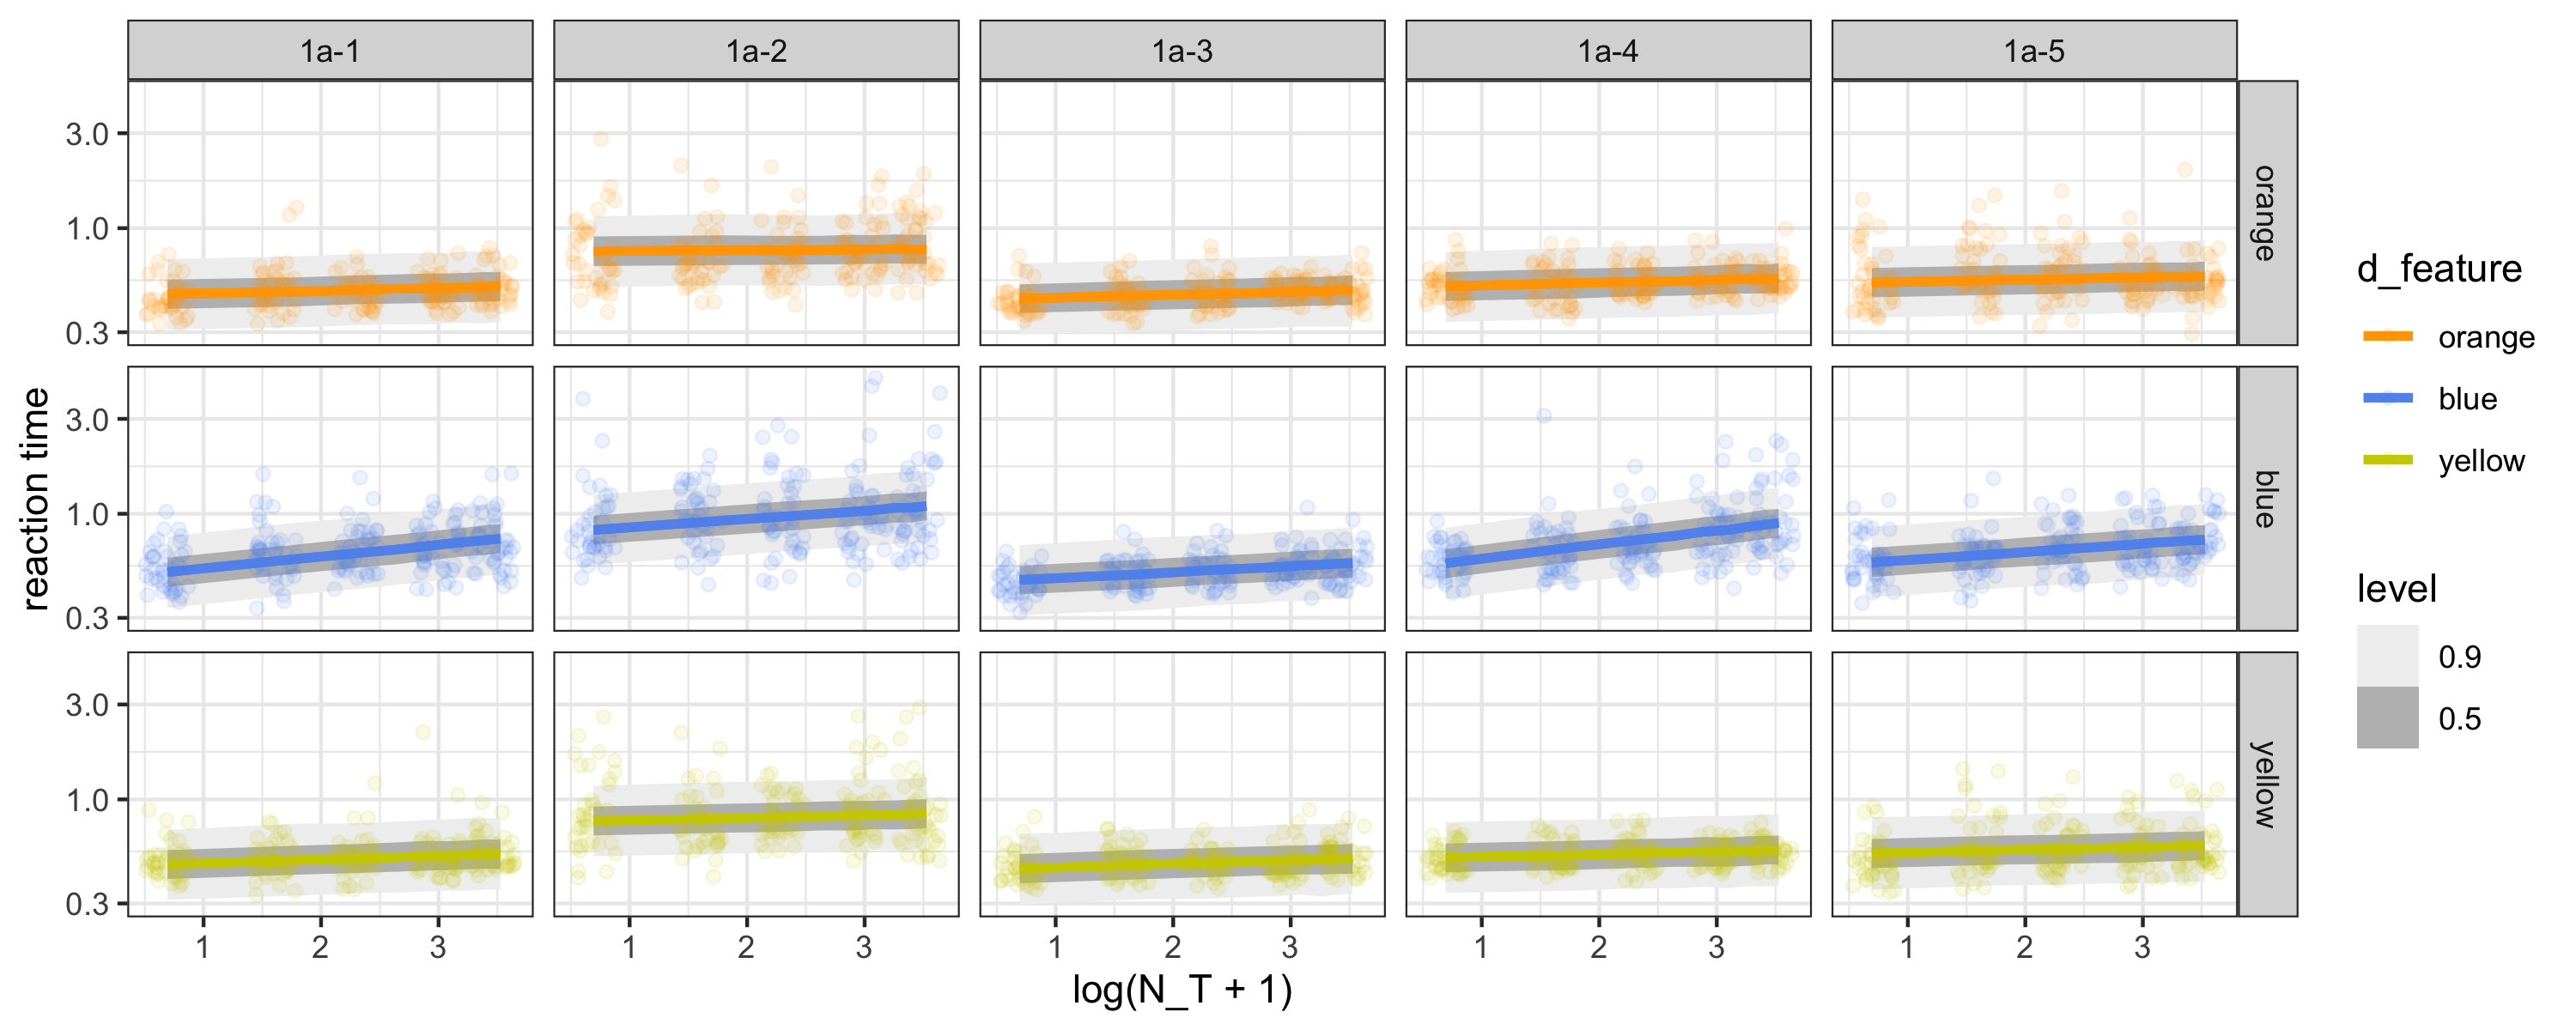
\includegraphics[width=\textwidth]{../reanalyse_Buetti2019/exp1_fits.png}}
\subfigure{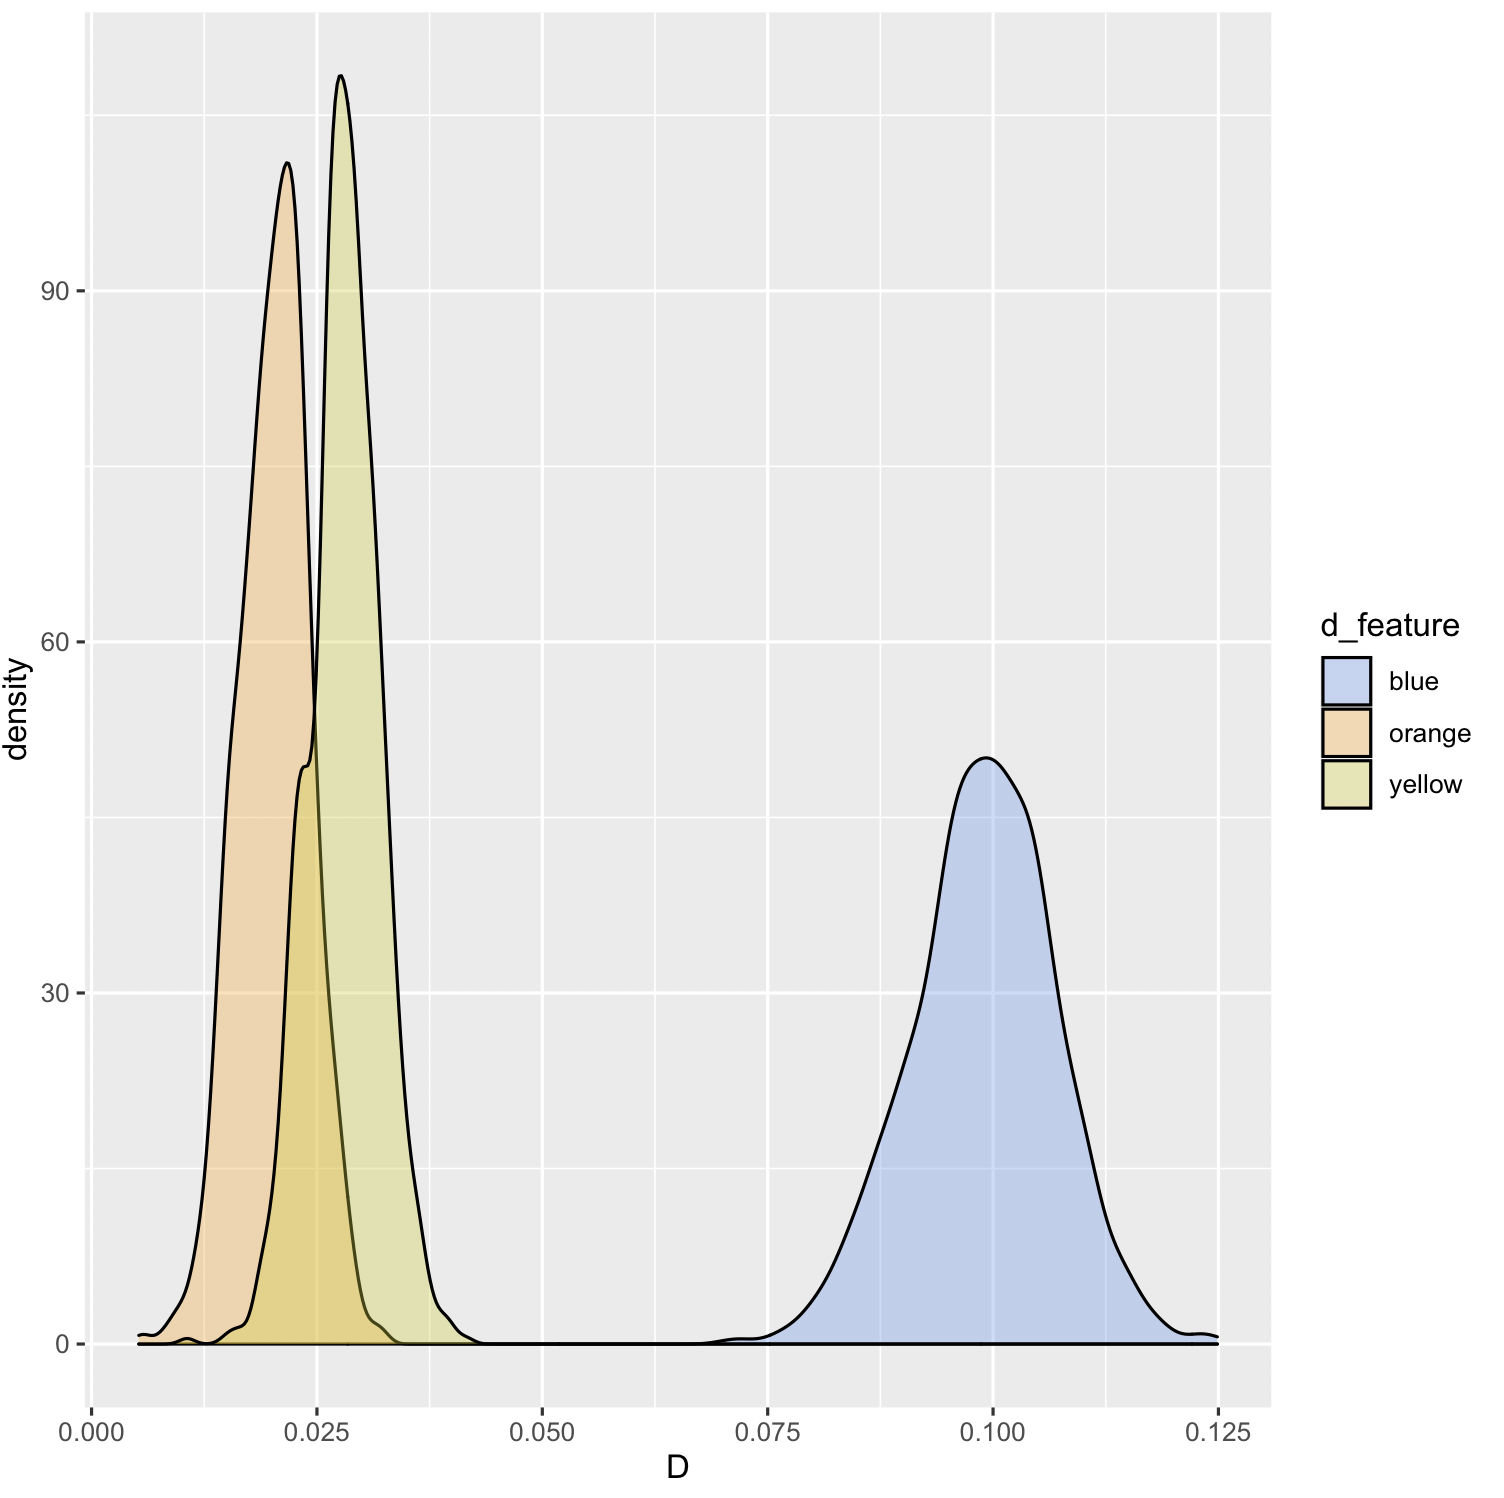
\includegraphics[width=\textwidth/0.4]{../reanalyse_Buetti2019/empirical_D_examples.png}}
\caption{Example results from the first five participants of Experiment 1a \cite{buetti2019predicting}. We can see considerable between-subjects variation. The shaded regions show the model's predicited reaction times.}
\label{fig:buetti2019_a1}
\end{figure}

\subsubsection{Fixed Effects}

As we are using a Bayesian framework, rather than $D$ representing the best fit in equation \ref{eq:computeDlm}, it is now represented as a probability distribution over possible values (see Figure \ref{fig:buetti2019_a1}.) We can can then estimate $D$ using the three methods and compare the predicted values to the empirical - see Figure \ref{fig:buetti2019_D}.

\begin{figure}
\centering
\subfigure{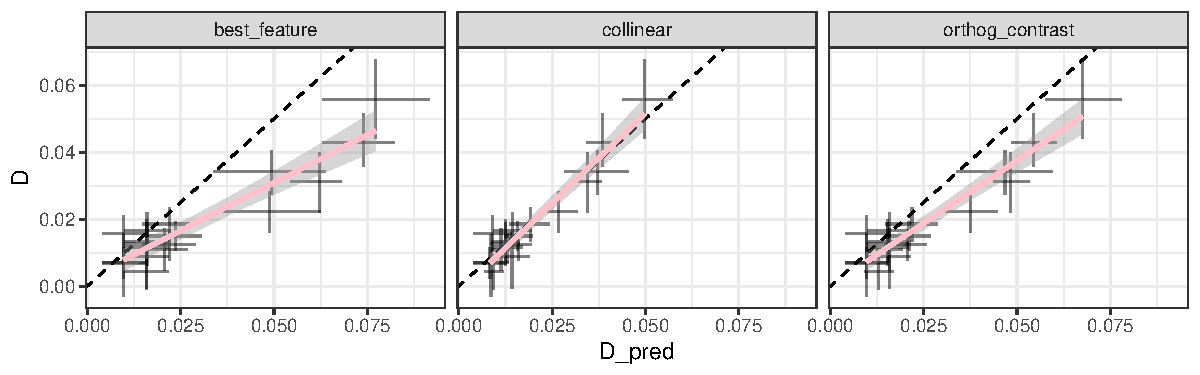
\includegraphics[width=\textwidth]{../reanalyse_Buetti2019/recreate_normal_fig_4.pdf}}
\subfigure{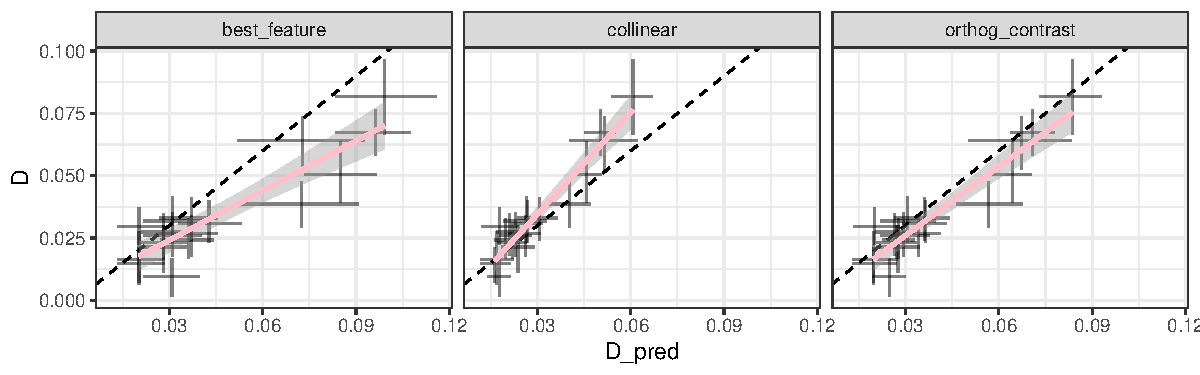
\includegraphics[width=\textwidth]{../reanalyse_Buetti2019/recreate_log_normal_fig_4.pdf}}
\caption{Correlation between empirical $D$ and the predicted $D$ using \textit{(top)} normal and (\textit{bottom}) log-normal distributions.}
\label{fig:buetti2019_D}
\end{figure}



\subsubsection{Individual Differences}


\subsection{Discussion}

It looks like, while we replicate the good predicitons using the colllinear method, we do not find this that this is the best method, and instead, we find the orthogonal contrast method is slightly better. 


\section{Experiment 1}

H0: confirm collinear method is best (compared to orthogonal contrast combination and best feature guidance models)

[If this is indeed the case, we will use only the collinear contrast integration model in the following experiments].

\subsection{Methods}

\subsection{Results}

\subsection{Discussion}



\begin{acknowledgements}
Thank you to AL for help and encouragement! 
\end{acknowledgements}


% Authors must disclose all relationships or interests that 
% could have direct or potential influence or impart bias on 
% the work: 
%
% \section*{Conflict of interest}
%
% The authors declare that they have no conflict of interest.


% BibTeX users please use one of
\bibliographystyle{plain}      % basic style, author-year citations
%\bibliographystyle{spmpsci}      % mathematics and physical sciences
%\bibliographystyle{spphys}       % APS-like style for physics
\bibliography{sources}   % name your BibTeX data base

% Non-BibTeX users please use
%\begin{thebibliography}{}
%
% and use \bibitem to create references. Consult the Instructions
% for authors for reference list style.
%
%\bibitem{RefJ}
% Format for Journal Reference
%Author, Article title, Journal, Volume, page numbers (year)
% Format for books
%\bibitem{RefB}
%Author, Book title, page numbers. Publisher, place (year)
% etc
%\end{thebibliography}

\end{document}
% end of file template.tex

